\subsubsection{Mobiiliverkko}
\begin{figure}[tb]
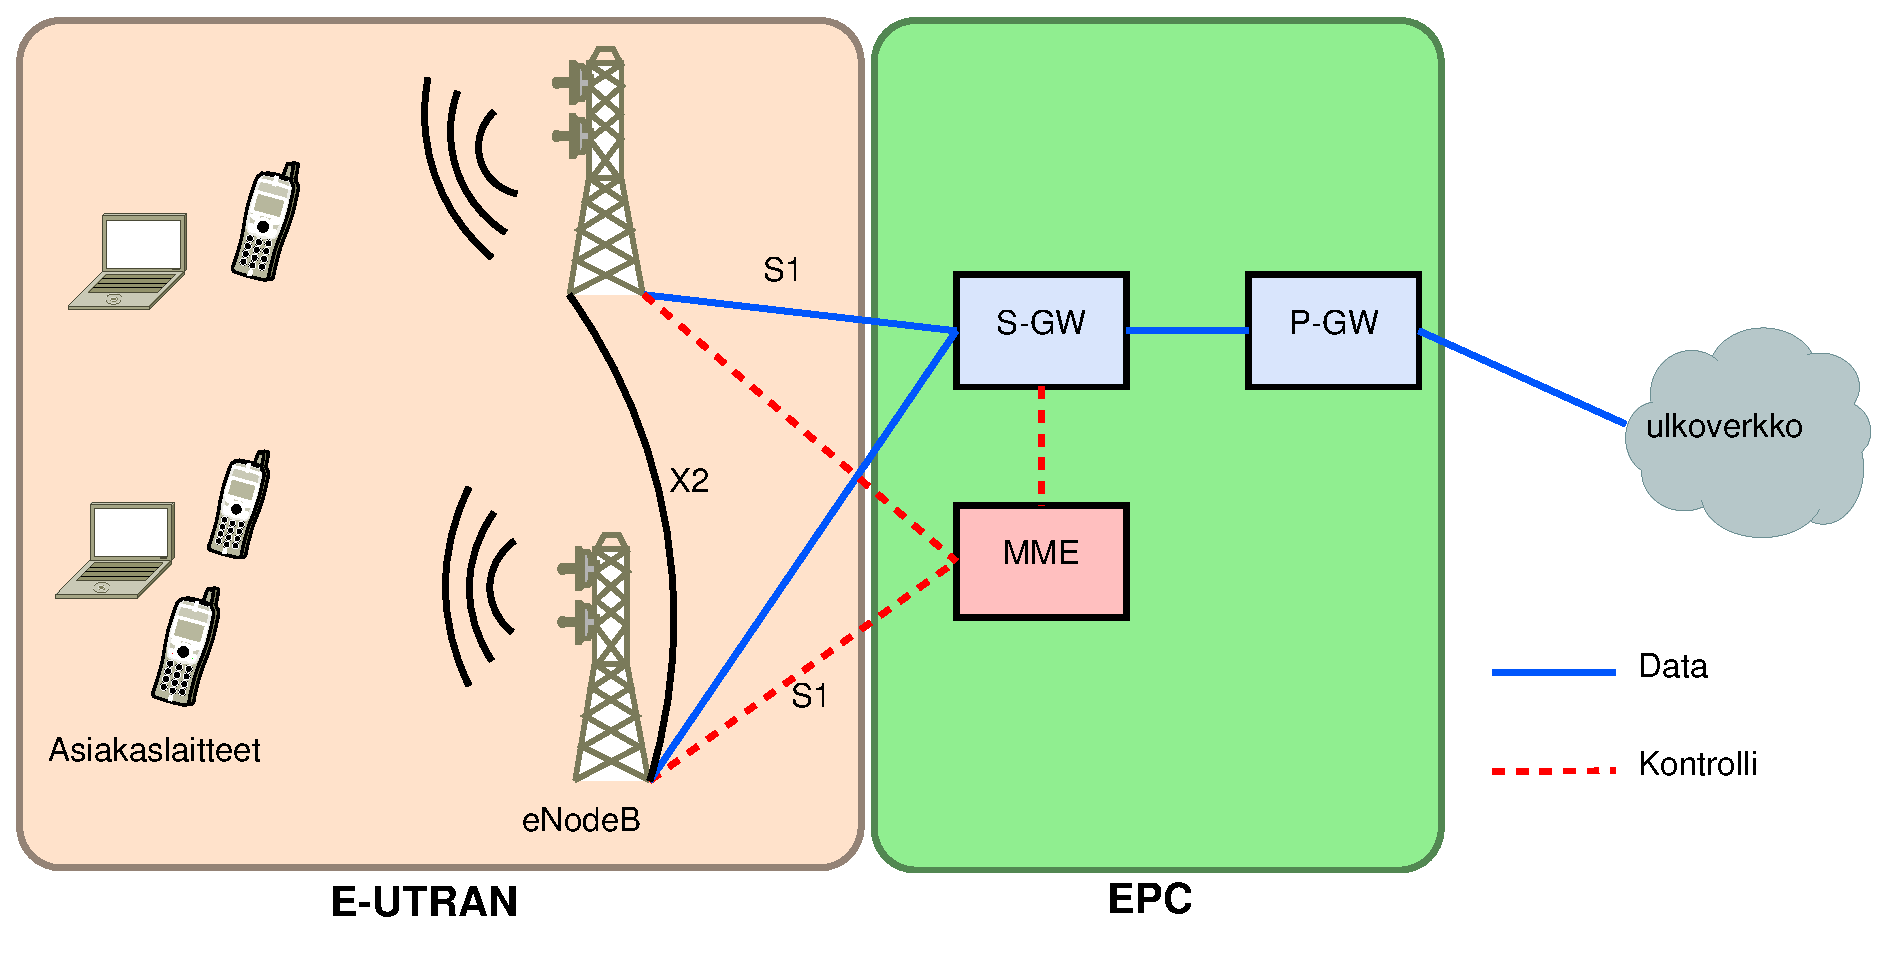
\includegraphics[width = \textwidth]{EPC.eps}
\caption{Yksinkertaistettu LTE-tyyppisen mobiiliverkon rakenne.} \label{fig:mobiarch}
\end{figure}

Tässä tutkielmassa käsiteltävät reuna-arkkitehtuurit sisältävät yhdistävänä tekijänä tavoitteen toimia mobiiliverkon yhteydessä. 
Täten reuna-arkkitehtuurien suunnittelupäätöksiä tarkasteltaessa on tarpeen ymmärtää mobiiliverkon osat yleisellä tasolla.
Yksinkertaisuuden vuoksi tämän tutkielman puitteissa mobiiliverkoksi oletetaan LTE:n mukainen arkkitehtuuri, joka koostuu E-UTRAN tyyppisestä radioverkosta ja EPC tyyppisestä runkoverkosta.
Seuraavaksi käydään läpi mobiiliverkon arkkitehtuurin tämän tutkielman kannalta merkitykselliset toimijat ja toiminnot.

Korkealla tasolla tarkasteltuna mobiiliverkko koostuu kahdesta osiosta: radioverkosta ja runkoverkosta. 3GPP kehittämässä LTE (Long Term Evolution) standardissa radioverkon sisältävä osuus on nimeltään E-UTRAN (Evolved UMTS Terrestrial Radio Access Network) ja runkoverkon osuus on nimeltään EPC (Evolved Packet Core).
E-UTRAN ja EPC väliset yhteydet on kuvattu kuvassa \ref{fig:mobiarch}.

E-UTRAN tehtävänä on toimia rajapintana asiakaslaitteen ja EPC:n välillä. 
E-UTRAN sisältää verkon puolella pääasiallisena toimijana eNodeB (Evolved nodeB) tyyppisiä tukiasemia \cite{etsieutran}.
Tukiasemista on olemassa muutamia erilaisia variaatioita, mutta tässä tutkielmassa käsitellään ainoastaan perustapausta.
Tukiasema on asiakaslaitetta lähimpänä sijaitseva funktionaalinen verkon osa ja sen seurauksena se on houkutteleva kohde reunalaskennan ratkaisuille. Tietoliikenteen näkökulmasta tukiaseman voi ajatella \textit{reunan} viimeisenä etappina ennen asiakaslaitteita. 

ENodeB tarjoaa asiakaslaitteiden suuntaan radioyhteyden.
EPC:n suuntaan eNodeB:t ovat yhteydessä S1 rajapinnan avulla.
Lisäksi eNodeB:t voivat olla toisiinsa yhteydessä X2 rajapinnan kautta.
S1:stä käytetään eNodeB:n ja EPC:n väliseen kommunikointiin. Tämä sisältää sekä hallinnollisen viestinnän, että asiakkaan tietoliikenteen kuljettamisen.
X2 rajapintaa puolestaan käytetään tukiasemien väliseen kommunikointiin. 
ENodeB välisten X2 yhteyksien tavoitteena on nopeuttaa tukiasemien välistä kommunikaatiota, esimerkiksi handoverin yhteydessä tehtävää asiakaskontekstin siirtoa varten \cite{3gpplte}.
Handoverilla tarkoitetaan asiakaslaitteen radioyhteyden siirtoa toiselle tukiasemalle. Handover käsitellään tarkemmin kappaleessa \ref{livemigraatio}.

Mobiiliverkon runkona toimiva EPC koostuu useista loogisista komponenteista.
Tämä siis tarkoittaa että toiminnallisuudet voivat fyysisesti sijaita samassa laitteessa. 
Tässä tutkielmassa on tarpeen ymmärtää perusteet seuraavista alikomponentista: MME (Mobility Management Entity), S-GW (Serving Gateway) ja PDN GW (P-GW, Packet data network gateway) \cite{etsilte}.
\begin{itemize}
\item \textbf{MME} on EPC:n hallinnollinen entiteetti joka vastaa muun muassa asiakaslaitteen tunnistamisesta ja handoveriin liittyvistä toimista EPC:n sisällä. Toisin kuin S-GW ja P-GW, MME ei käsittele asiakaslaitteiden tietoliikennettä.
\item \textbf{S-GW} eli palveluyhdyskäytävä toimii asiakaslaitteen EPC:n sisäisenä kiintopisteenä.  S-GW reitittää asiakaslaitteen liikennettä P-GW:n ja E-UTRAN välillä.
\item \textbf{P-GW} eli pakettiverkon yhdyskäytävän tehtävänä on toimia asiakaslaitteen ja mobiiliverkon ulkopuolisten IP-verkkojen yhteyspisteenä.
\end{itemize}
\cite{3gppepc}

Mobiiliverkossa käytävä kommunikaatio voidaan jakaa kahteen kerrokseen: kontrollikerrokseen ja tietoliikennekerrokseen.
Kontrollikerroksella välitettävät viestit ovat tarkoitettu hallinnollisiin toimintoihin mobiiliverkon sisällä. 
Tietoliikennekerros välittää asiakkaan tietoliikennettä internetin ja asiakaslaitteen välillä.
Asiakkaan tietoliikenne kulkee tukiaseman ja P-GW:n välillä GTP-tunneloituna (GPRS Tunnelling Protocol) \cite{puente15seamless}. Tämä tarkoittaa että mobiiliverkon sisällä tietoliikennettä ei ohjata asiakaslaitteen tietoliikenteen tunnisteiden pohjalta. 
